% =========================================================
% CONFIGURACION DEL DOCUMENTO
% =========================================================
\providecommand{\main}{..}
\documentclass[../main.tex]{subfiles}

% =========================================================
% CONTENIDO
% =========================================================
\begin{document}		
\chapter{Estado del arte}
\label{cha:02_estado_del_arte}

	\begin{figure}[H]
		\centering
		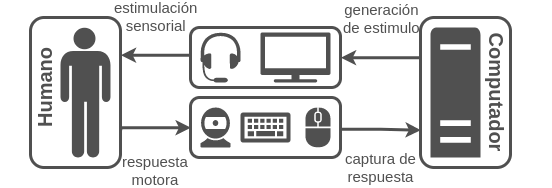
\includegraphics[width=0.8\textwidth]{cap_02_diagram}
		\caption{Diagrama general de la interfaz hombre-máquina.}
		\label{fig:02_diagrama_interfaz}
	\end{figure}

	\begin{figure}[H]
		\centering
		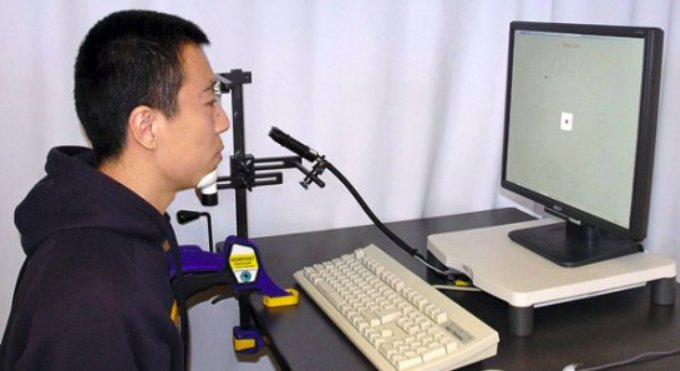
\includegraphics[width=0.5\textwidth]{cap_02_setup}
		\caption{Ejemplo de setup experimental \cite{website:baseInfo}.}
		\label{fig:02_ejemplo_setup}
	\end{figure}

	\section{Sistemas de seguimiento ocular}
	\label{sec:02_sistemas_de_seguimiento_ocular}
		\subsection{Movimiento ocular}
		\label{sub:02_movimiento_ocular}

		La acción de dirigir la mirada hacia un objeto es parte fundamental del proceso de visión. Este acto involucra el direccionamiento de los ejes visuales\footnote{Corresponde a la proyección de una línea recta que pasa simultáneamente por el centro de la fóvea, área de la retina que permite la visión más nítida y detallada, y la pupila.} hacia un objetivo determinado, permitiendo la realización de análisis visuales precisos. Dicha orientación muchas veces implica movimientos coordinados de los ojos, cuello y cabeza, no obstante, existen movimientos más pequeños que son realizados únicamente por los ojos, conocidos como movimientos sacádicos \cite{article:movOcular, website:movOcular}.

		Los movimientos sacádicos corresponden a las rotaciones que realiza el globo ocular entre dos momentos de posicionamiento estacionario, cabe indicar que durante estos no se obtiene información visual relevante. Para individuos en condiciones normales este tipo de movimiento se realiza constantemente y se repite varias veces por segundo, el direccionamiento de los ojos en estos casos suele ser controlado por procesos cognitivos realizados de forma inconsciente.

		Las características principales de dichos movimientos son:
		\begin{enumerate}
			\item Cada sacada tiene un patron de movimiento similar, por lo tanto son altamente caracterizables.

			\item Por su naturaleza los movimientos sacádicos son denominados balísticos, esto quiere decir que la posición de destino se encuentra predeterminada en el momento de partida. 

			\item La velocidad de las sacadas aumenta de forma no lineal en la medida que aumenta la amplitud de movimento (cosa que se cumple bajo toda circunstancia). De esta forma la duración del movimiento puede fluctuar entre $20 - 100[ms]$ y sus velocidades entre $10 - 300 [\frac{deg}{s}]$.

			\item La precisión del movimiento sacádico fluctúa entre un $5-10\%$ de la amplitud total y las correcciones son realizadas por movimientos de calibración denominados micro-sacadas. Estos métodos correctivos permiten suponer que existe algún tipo de procesamiento paralelo encargado de la calibración ocular de largo plazo \cite{website:movOcular}.  

		\end{enumerate}

		Las características expuestas entregan, a grandes razgos, nociones que permiten comprender el por qué su estudio se ha vuelto común en campos científicos como la neurociencia: Dado que los movimientos del globo ocular son caracterizables, de patrones definidos y de alta presición es posible identificar mediante ellos enfermedades neurodegenerativas, que tienden a alterar los comportamientos motrices. Un ejemplo de esto es la enfermedad de Parkinson, donde una afección crónica a los ganglios basales produce una reducción progresiva de la sustancia negra lo que se traduce en una producción insuficiente de dopamina, neurotransmisor relevante para la función motora; Esta insuficiencia se traduce en aumentos en los tiempos de respuesta y tasas de error en diversas tareas (ver \ref{sub:02_experimentos_de_estimulacion}) asociadas a movimiento ocular.    

		\subsection{Métodos de captura}
		\label{sub:02_metodos_de_captura}
			\subsubsection{Un poco de historia}
			\label{ssub:02_un_poco_de_historia_tracker}

			El estudio y registro de los movimientos oculares tiene sus inicios a principio del siglo XVIII donde, mediante espejos, telescopios y mirillas estudiosos observaban los comportamientos oculares de pacientes y sujetos de prueba. Aún que sus conclusiones y descubrimientos dieron un puntapié inicial a estudios posteriores no fue hasta finales del mismo siglo cuando, de la mano de instrumentos mécanicos, investigadores tuvieron la oportunidad de registrar de forma objetiva dichos movimientos, pudiendo así tener un respaldo real de las características detectadas \cite{article:eyetracker_eggert}.

			De esta forma, los primeros métodos de captura o eye trackers se encontraban no solo limitados por la tecnología existente en la época, sino, por la capacidad del individuo que registraba de describir correctamente los resultados. 

			A principios del siglo XX Delabarre (1898) \cite{article:eyetracker_richardson} fue capaz de utilizar un sistema de palancas 
			A finales del siglo XIX y principalmente de la mano de estudios psicológicos se   no obstante sus conclusiones no poseían mayor respaldo  A pesar de Estos métodos por supuesto, altamente dependientes de las consideraciones y sesgos de quienes realizaban los experimentos 
			En  se indica que el estudio del ojo 

			\subsubsection{Tecnologías actuales}
			\label{ssub:02_tecnologias_actuales}
				\begin{enumerate}
					\item \textbf{De contacto directo}

					\item \textbf{Seguimiento ocular}

					\item \textbf{Medición de potencial eléctrico}

				\end{enumerate}

			\subsubsection{Comparativa}
			\label{ssub:02_comparativa_eyetracker}
			
		\subsection{Sistemas comerciales más relevantes}
		\label{sub:02_sistemas_comerciales_más_relevantes}
			\begin{enumerate}
				\item \textbf{EyeGaze}

				\item \textbf{EyeLink}

				\item \textbf{EyeTribe}

				\item \textbf{IViewX}

				\item \textbf{Tobii}

			\end{enumerate}

	\section{Sistemas de estimulación visual}
	\label{sec:02_sistemas_de_estimulacion_visual}
		\subsection{Hardware de estimulación}
		\label{sub:02_hardware_de_estimulacion}
			\subsubsection{Un poco de historia} 
			\label{ssub:02_un_poco_de_historia_monitores}

			A lo largo de la historia las tecnologías utilizadas 

			\subsubsection{Tecnologías actuales} 
			\label{ssub:02_tecnologias_actuales}
				\begin{enumerate}
					\item \textbf{Monitores CRT}

					\item \textbf{Monitores LED, oLED, LCD}

				\end{enumerate}

			\subsubsection{Comparativa}
			\label{ssub:02_comparativa_monitores}
			
		\subsection{Software de estimulación}
		\label{sub:02_software_de_estimulacion}
			\subsubsection{Software más relevante}
			\label{ssub:02_software_mas_relevante}
				\begin{enumerate}
					\item \textbf{PsychoPy}

					\item \textbf{PsychoToolbox}

					\item \textbf{VissionEgg}

					\item \textbf{Presentation}

				\end{enumerate}

			\subsubsection{Comparativa}
			\label{ssub:02_comparativa_software}

		\subsection{Experimentos de estimulación}
		\label{sub:02_experimentos_de_estimulacion}

		Las tareas mencionadas con anterioridad \cite{article:tests_1, article:tests_2} se encuentran diseñadas para evaluar uno o más de los siguientes tipos de movimiento sacádico:
		\begin{enumerate}
		 	\item \textbf{Movimiento reflexivo:}

		 	\item \textbf{Movimiento voluntario:}
		 	
		 	\item \textbf{Movimiento pro-sacádico:}
		 	
		 	\item \textbf{Movimiento anti-sacádico:}

		 	\item \textbf{Movimiento retardado:}

		 	\item \textbf{Movimiento guiado por memoria:}

		 	\item \textbf{Movimiento microsacádico:}

		 \end{enumerate} 

		 Que pueden presentar modificaciones para ajustarse a alguno de los siguientes paradigmas:
		 \begin{enumerate}
		 	\item \textbf{Efecto de gap:}

		 	\item \textbf{Efecto de distractor:}

		 	\item \textbf{Efecto de inhibición sacádica:}

		 \end{enumerate}


		 Que se traducen en información asociable a alguna métrica determinada. A continuación se describen algunas de ellas:
		 \begin{enumerate}
		 	\item \textbf{Latencia sacádica (SL):}

		 	\item \textbf{Intervalo inter-sacádico (ISI):}
		 	
		 	\item \textbf{Ganancia inicial de movimiento:}
		 	
		 	\item \textbf{Tasa de error:}

		 \end{enumerate} 

\end{document}
